%---
\subsection{The \DSk\ Liquid Argon Time Projection Chamber}
\label{sec:TPC}


%---
\paragraph{\LArTPC\ Size Consideration}
% some numbers are updated in this subsection

Since the \SiPM\ tiles are all square shape, the \DSk\ \TPC\ will be an octagonal shape to best fit the coverage of the photo detector module (\DSkPdm) while optimizing the fiducial mass. 
The size of the \TPC\ is determined by the patterning strategy of the \SiPMs, driven by the design size of the square and triangular Motherboards (SQB and TRB, respectively).  Figure~\ref{fig:TPC-SiPM_pattern} shows the current \SiPM\ pattern strategy for both top and bottom array, each array consists of \DSkArraySQBNumber\ \SQBs\ and \DSkArrayTRBNumber\ \TRBs. Each \TRB\ contains \DSkTRBPdmsNumber\ \DSkPdms\ and each \SQB\ contains \DSkSQBPdmsNumber\ \DSkPdms.  Thus, the number of \DSkPdms\ used in each array is \DSkTilesHalfNumber, and the total number of \DSkPdms\ used in the \TPC\ is \DSkTilesNumber.  Based upon this pattern strategy, considering that the edge of the active volume of the \TPC\ will shrink about \SI{10}{\centi\meter} from the edge of the \SiPM\ array, to maximize the coverage of the photon detectors the distance from edge to edge of the octagonal active volume is \SI{3.5}{\meter}.  The height of the \TPC\ is \SI{2.63}{\meter}. With this design, the total mass of \LAr\ in the active volume and fiducial volume (with 10-cm cut, both vertically and laterally) are \DSkActiveMass\ and \DSkFiducialMass\, respectively. 
\begin{figure}[h!]
\centering
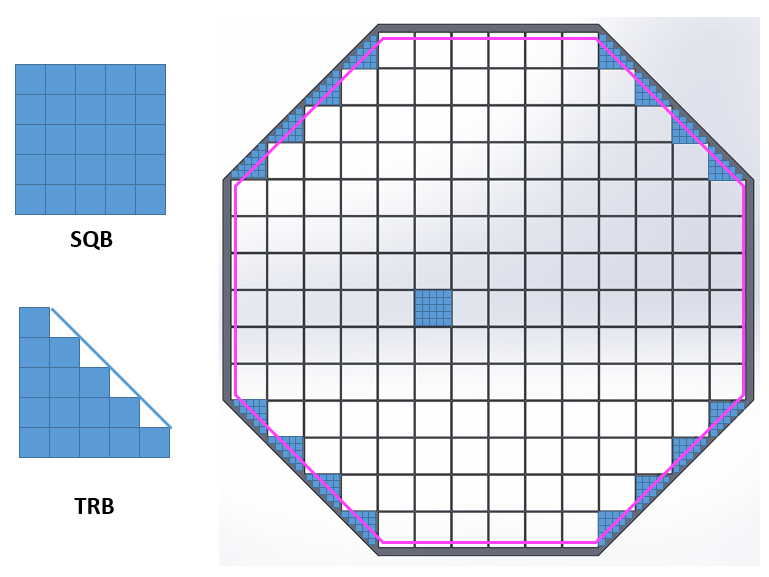
\includegraphics[width=\columnwidth]{Figures/TPC-SiPM_pattern.png}
\caption{Patterning scheme for the \DSkPdms. Pink lines indicate the edges of \TPC\ active volume.}
\label{fig:TPC-SiPM_pattern}
\end{figure} 

%---
\paragraph{Reflector Panel}
% a paragraph of PTFE and ESR reflection comparison measurement is added in this subsection

In order to get rid of the conventional \PTFE, which would be the predominant source of neutron background and Cherenkov background by its enormous mass required in \DSk, the Enhanced Specular Reflector (ESR,~\cite{ESR}) foil will be used as the \TPC\ reflector. ESR is a thin layer foil which has reflectivity for \DSfPMTWaveLength\ light, up to \SI{98}{\percent}, with a thickness of only \SI{65}{\micro\meter}.  To hold the ESR foil in place and maintain its flatness during the operations, two pieces of UVT acrylic sheets are used to sandwich the ESR foil in the middle. The acrylic sheet facing to the active \LAr\ volume is chosen to be only \SI{1}{\mm} thick, in order to minimize the Cherenkov light introduced by itself, while the thickness of the backside acrylic sheet is chosen to be \SI{4}{\mm}, strong enough to hold the entire sandwich. Almost all Cherenkov light introduced by this acrylic sheet and any other material outside will be blocked by the ESR foil. The surface of each \SI{1}{\mm} thick acrylic sheet facing the active \LAr\ volume is coated with \TPB.

\begin{figure}[h!]
\centering
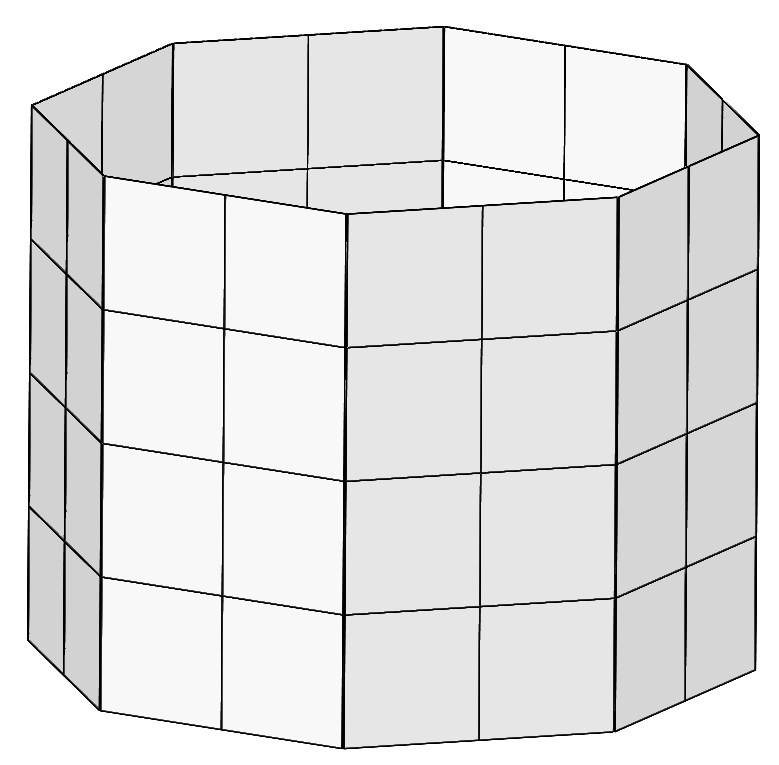
\includegraphics[width=\columnwidth]{./Figures/TPC-reflector_panel.png}
\caption{3D model of the full \DSk\ \LArTPC\ reflector panel.}
\label{fig:re_panel}
\end{figure}

\begin{figure}[h!]
\centering
\includegraphics[width=\columnwidth]{./Figures/TPC-reflector_corner.png}
\caption{Cross-sectional view of the reflector panel corner joints.}
\label{fig:re_corner}
\end{figure}

The entire reflection panel of the \TPC\ is shown in Figure~\ref{fig:re_panel}. There are two different kinds of ESR-acrylic sandwiches, the flat assembly and the corner assembly. Each ESR-acrylic sandwich assembly is fixed by several \PTFE\ screws, with the screw heads facing to the active volume. In order not to lose any light, each head of the \PTFE\ screw is coated with \TPB\ as well. Some space is left between the acrylic and the ESR to allow venting of any gas during filling of the \LAr, and also to allow \LAr\ to fill the space and reduce the chances for total internal reflection of light within the ESR-acrylic sandwich.
The flat assemblies and the corner assemblies are mounted on the field cage, which is holding by another set of acrylic structures, by the \PTFE\ screws, but the corner assemblies and the flat assemblies are not directly connected to each other in order to accommodate the shrinkage when the assemblies are immersed in the \LAr\, as shown in Figure~\ref{fig:re_corner}. Overlaps between ESR foils at each joint are also designed for the same reason. A small mockup to mimic the shrinkage has been built at UC Davis. Repeated tests in liquid nitrogen showed that all parts moved in the desired way during cooling down and warming up, which proves the design idea.

%---
\paragraph{Field Region}
% some numbers are updated in this section, the idea of replacing the copper rings by the conductive polymer coating is mentioned as new stuff.

The relative permittivity of \LAr\ and gaseous argon are \num{1.54} and \num{1.03}, respectively.  By applying ground, \SI{-3.78}{\kV}, and \SI{-52.6}{\kV} to the anode, extraction grid and cathode, respectively, three different fields are formed in the \TPC:

\begin{compactitem}
\item The drift field of \SI{200}{\V\per\cm} in the liquid phase is made uniform by the design of the field cage. The drift distance between the cathode \ITO\ layer and the extraction grid is \SI{263}{\cm};
\item The extraction field in the liquid phase above the grid is \SI{2.8}{\kV\per\cm}. The distance between the extraction grid and the surface of the \LAr\ is \SI{3}{\mm};
\item The electroluminescence field in the gas phase is \SI{4.2}{\kV\per\cm}. The gas gap between the surface of the \LAr\ and the \ITO\ layer acting as the anode is \SI{7}{\mm} thick.
\end{compactitem}

As the top boundary of the active volume, a \DSkPMMATPCThickness thick acrylic window serves as the diving bell to maintain a stable gas pocket. A thin layer of \ITO\ is coated on the bottom surface as the anode, and a layer of the \TPB\ will be coated on the \ITO\ layer.
The \ITO\ layer extends beyond the gas pocket edge, as shown in Figure~\ref{fig:TPC_anode}, in order to improve the uniformity of the electroluminescence field near the edge. Right below the acrylic diving bell is the extraction grid, composed of stainless steel wires stretched in parallel with \SI{3}{\mm} spacing on a stainless steel frame. Radial slots on the rim of the acrylic diving bell act as concentric guide, to compensate the different thermal expansion coefficients between acrylic and stainless steel.
The \LAr\ level will be maintained at the top surface of the grid frame.
Suitable tensions will be pre-loaded on each of the grid wires to minimized the sagging, an effect that will distort the electroluminescence field. The frame must be stiff enough to sustain the total force of all wires, while remaining not too bulky. Both simulation studies and prototype tests are being performed at Houston to optimize the grid design.

\begin{figure}[h!]
\centering
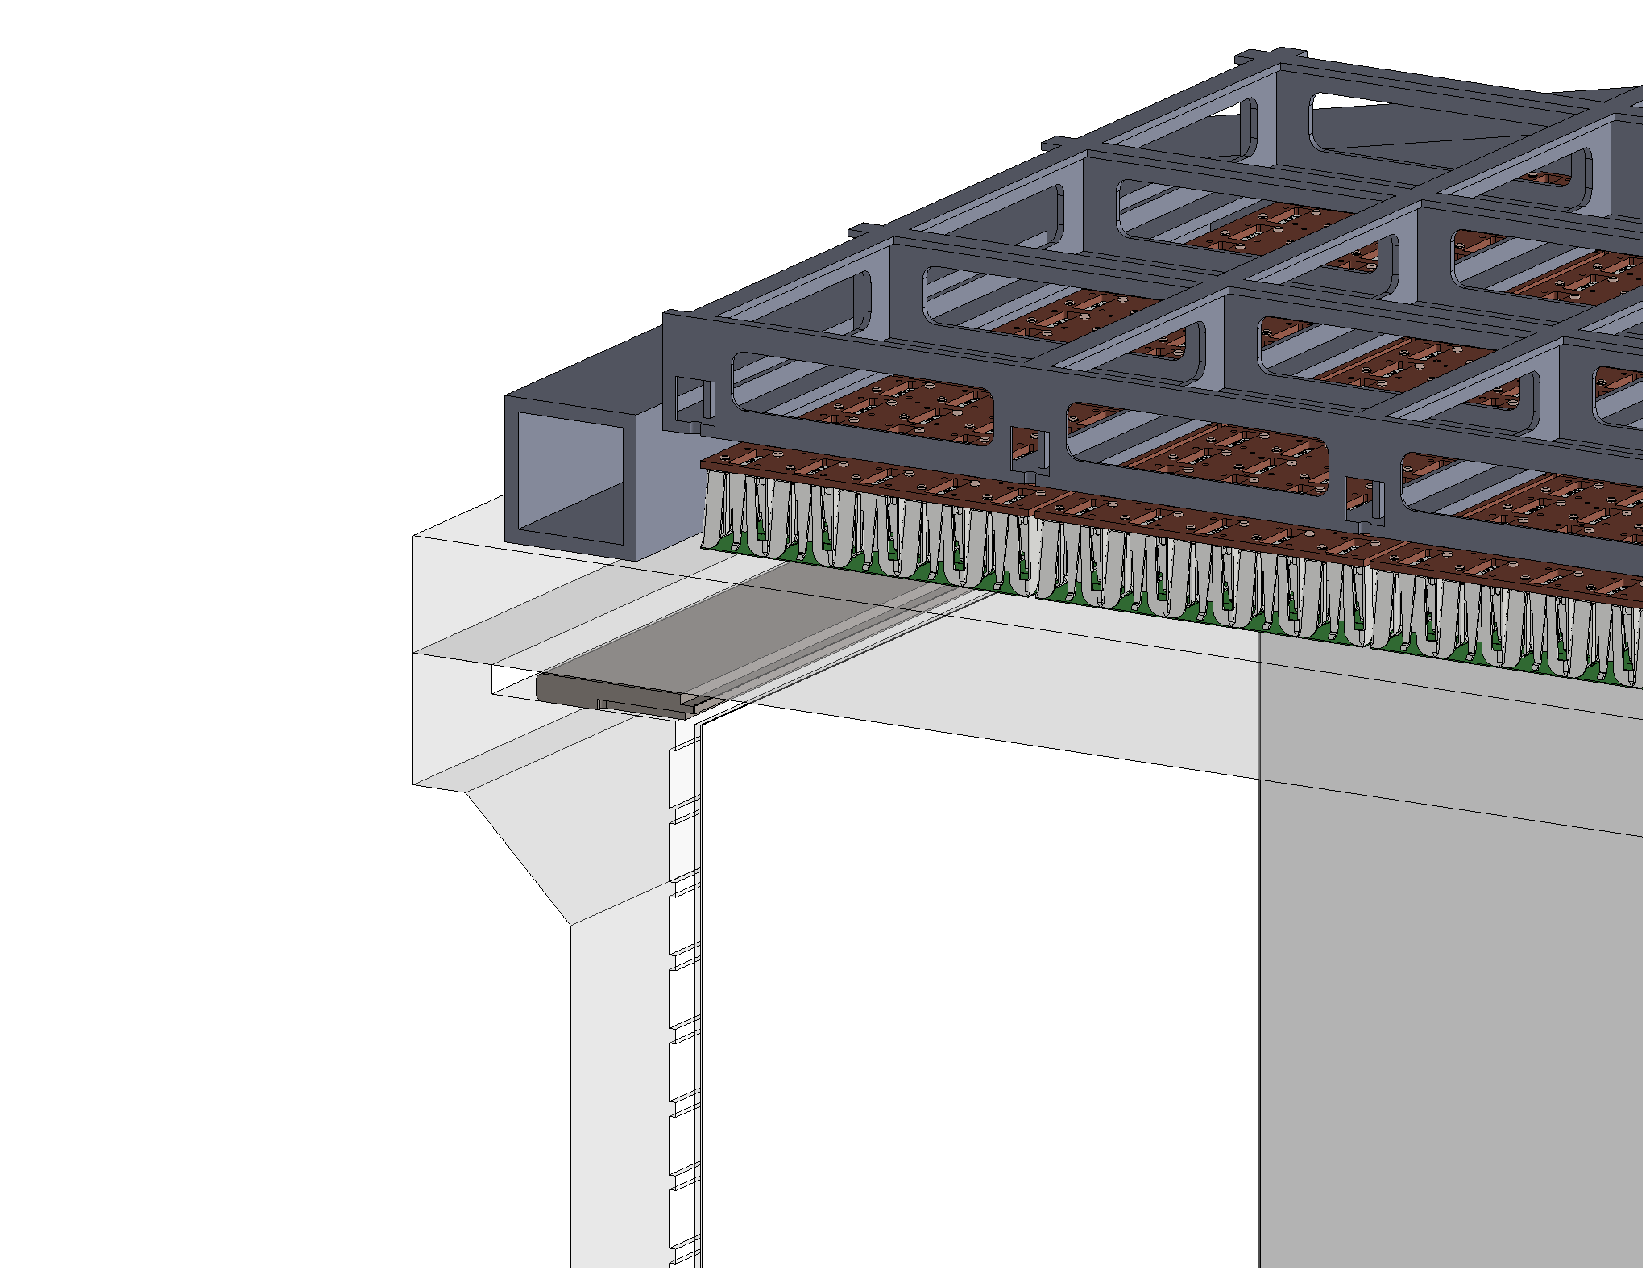
\includegraphics[width=\columnwidth]{./Figures/TPC-anode.png}
\caption{3D model of the \LArTPC\ anode and extraction grid region.}
\label{fig:TPC_anode}
\end{figure}

The bottom boundary of the active volume, shown in Figure~\ref{fig:TPC_cathode}, is a \DSkPMMATPCThickness\ thick acrylic window coated with a thin layer of \ITO\ on both side. A layer of \TPB\ will be coated on the top \ITO\ layer of the cathode acrylic window for wavelength shifting. The edge of the top ITO layer contacts with a C-profile guard copper ring to smooth the electric field lines. This ring delivers the \SI{-52.6}{\kV} to cathode and minimizes the electric field at the edge of ITO layer. Similarly, the bottom \ITO\ layer contacts with a P-profile solid guard copper ring, for ground delivery and electric field minimization. The acrylic window can easily sustain the applied electric field with this design. Besides minimizing the electric field at the edge of ITO layer, in order to avoid discharge between the cathode ITO layer and the ground ITO layer in the liquid argon, a pattern of grooves are machined on the non-coated area at the edge of the cathode acrylic window. 
Free surface charges created during the detector operation will be trapped within the grooves. This design prevents the discharge caused by the motion of surface charges.
This concept was tested to be electrically stable up to about \SI{-65}{\kV} with a full-scale mockup of the \DSf\ cathode region, using a \SI{6.5}{\mm} thick fused silica window in an open dewar. 
In order to avoid accumulation of the bubbles generated by the bottom photon detector array or any other parts, the bottom surface of the cathode acrylic windows will be a convex instead of a flat surface.

\begin{figure}[h!]
\centering
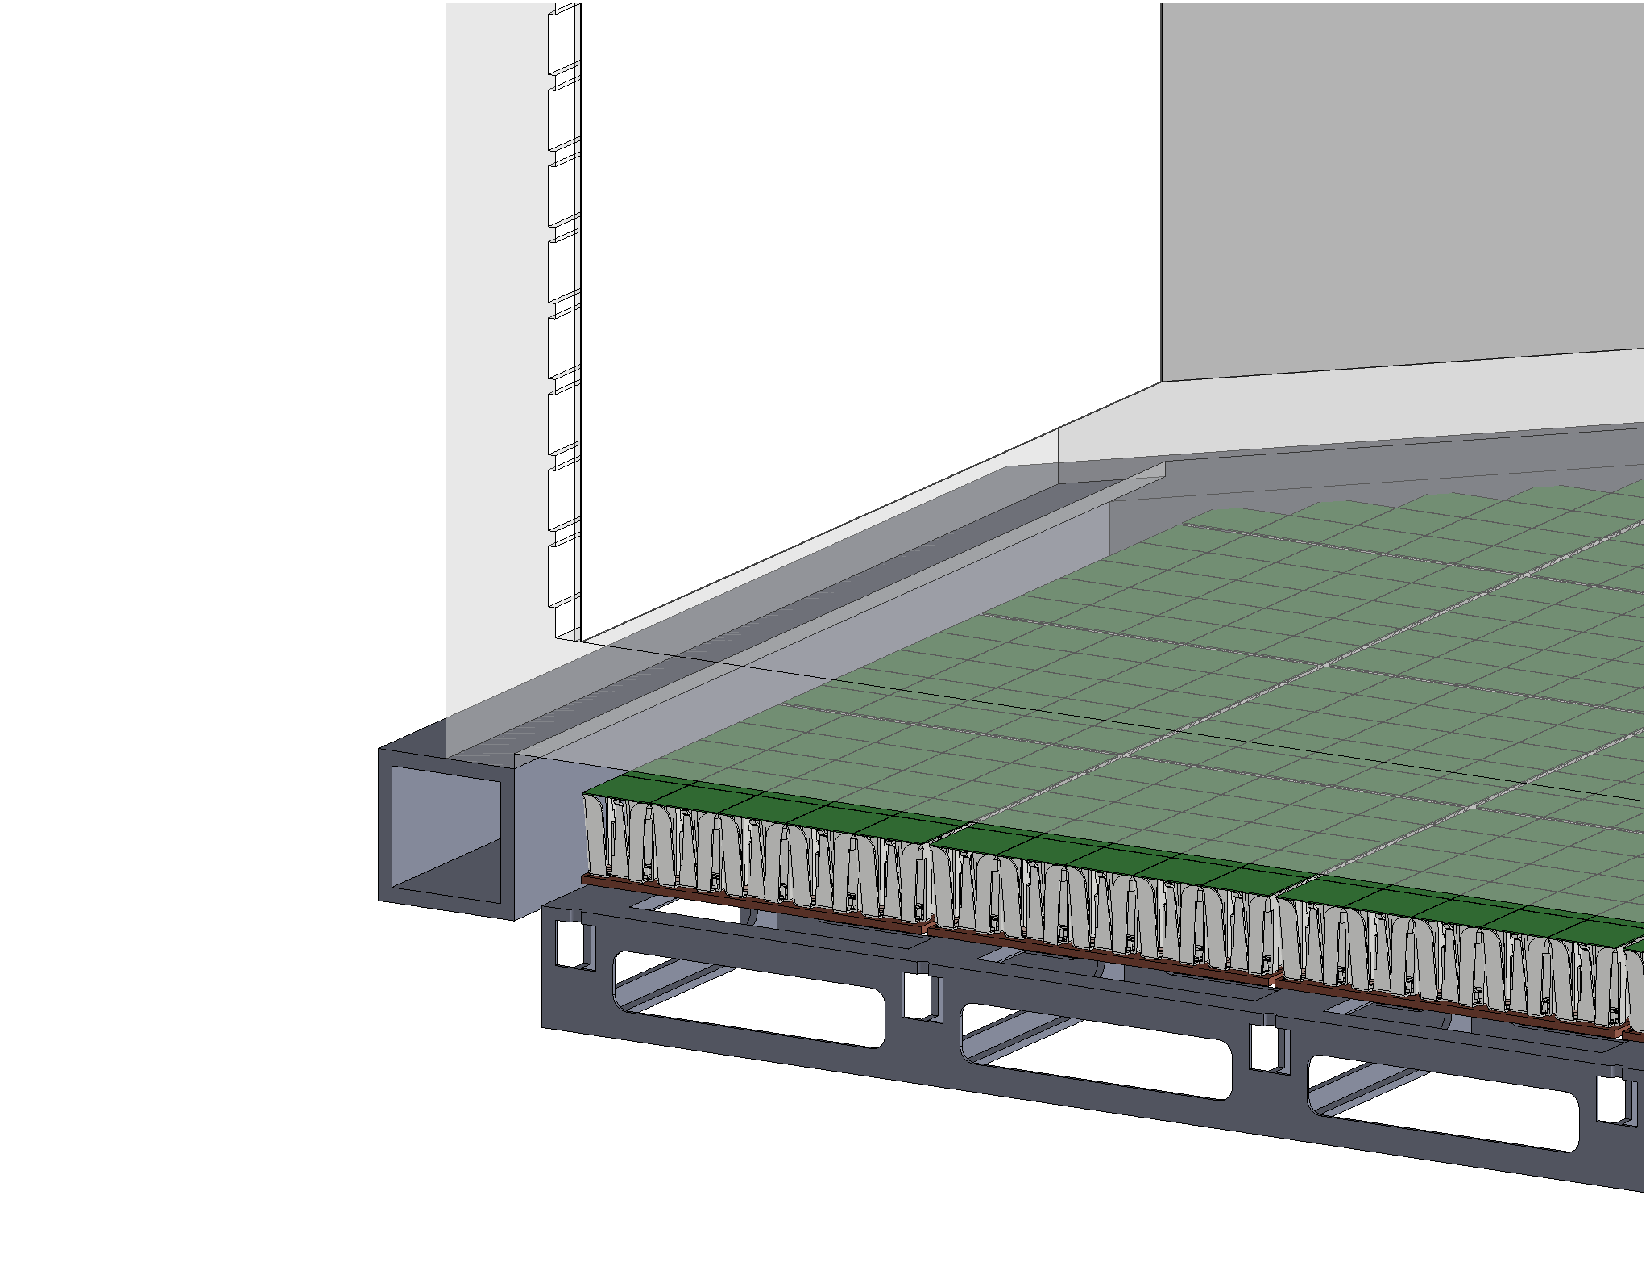
\includegraphics[width=\columnwidth]{./Figures/TPC-cathode.png}
\caption{3D model of the \LArTPC\ cathode region.}
\label{fig:TPC_cathode}
\end{figure}

A commercial conductive and transparent Polymer coating, Clevios~\cite{Clevios}, is found to be a very promising alternative of \ITO. Clevios is being used in industrial applications such as transparent electrodes for touch panels and printed electronics. The main advantage for us is that Clevios is a water-based solution, so a large-area coating needed for anode and cathode is easier to accomplish than \ITO\ coating.
A sample of \SI{100}{\gram} has been purchased for the radioactivity assay. The initial ICP-MS assay results from PNNL are encouraging, and further analysis of Rn emanation is scheduled at Krakow. In terms of the optics, three coating samples of Clevios on acrylic plates are provided by Heraeus. The coating thickness of each sample is \SI{4}{\um}, \SI{8}{\um} and \SI{12}{\um}, respectively, and the transparency has been measured at Princeton. About \SI{1.5}{\percent} absorption at \DSfPMTWaveLength\ contributed by \SI{4}{\um} thick Clevios layer was observed, which is very good compared with \ITO. We are keeping in contact with Heraeus to understand the coating process in detail, and more Clevios samples are being ordered by CERN. Besides the anode and cathode, the bulky Cu field shaping rings may also be replaced by Clevios coatings.
Consequently, it may reduce the background as well as the total cost, and make the fabrication and installation of the \TPC\ simpler. More investigations are being performed in this direction.


%---
\paragraph{Acrylic Vessel}
% the section of copper vessel is removed, and replaced by this section

In current design as described above, the \TPC\ active volume is confined by acrylic plates or panels from all directions. In order to utilize \UAr\ more efficiently, all the \UAr\ will be sealed in this acrylic vessel and no other external vessel is required, as shown in Figure~\ref{fig:TPC_acrylic}. 
The body of the acrylic vessel is fused together by \DSkPMMATPCThickness\ thick acrylic plates, and then flanged and sealed with the 
%top lid which is another \DSkPMMATPCThickness\ thick acrylic plate. The
 top and the bottom lid, that  serve as the anode plate and cathode plate of the \TPC, respectively. 
%In this case, the design for anode region and cathode region as described above (Figure~\ref{fig:TPC_anode} and Figure~\ref{fig:TPC_cathode}, respectively) will be simplified and bulky components will be further avoided, resulting in a reduced background from \TPC\ material.
The ESR-acrylic sandwich reflection panels are located inside the acrylic vessel. The top and bottom \DSkPdm\ arrays are placed outside of the acrylic vessel, immersed in the \AAr\ of the veto detector. \DSkPdm\ arrays will be well covered and isolated from light of the veto detector.
In this way, 
%partially acts as \TPC, and 
the entire volume inside the acrylic vessel  is active, resulting in the most efficient usage of \UAr. All cables and HVFTs and most mechanical structures are now moved outside of the \UAr\ volume as well, resulting in less outgassing hence higher purity of \UAr. 

The HV Cathode connection through the acrylic vessel is being studied and a new design will be tested to adapt the HV cable connection to the cathode. The acrylic vessel design integrate the HV connection so that the contact point is outside the vessel and already sealed with the \UAr. In this case, both the HV Cable and the \HVFT\ are in the \AAr\ volume, and the \HVFT\ is going through the veto cryostat, becoming the standard connection which has been tested repeatedly in previous DarkSide programs. 

\begin{figure}[h!]
\centering
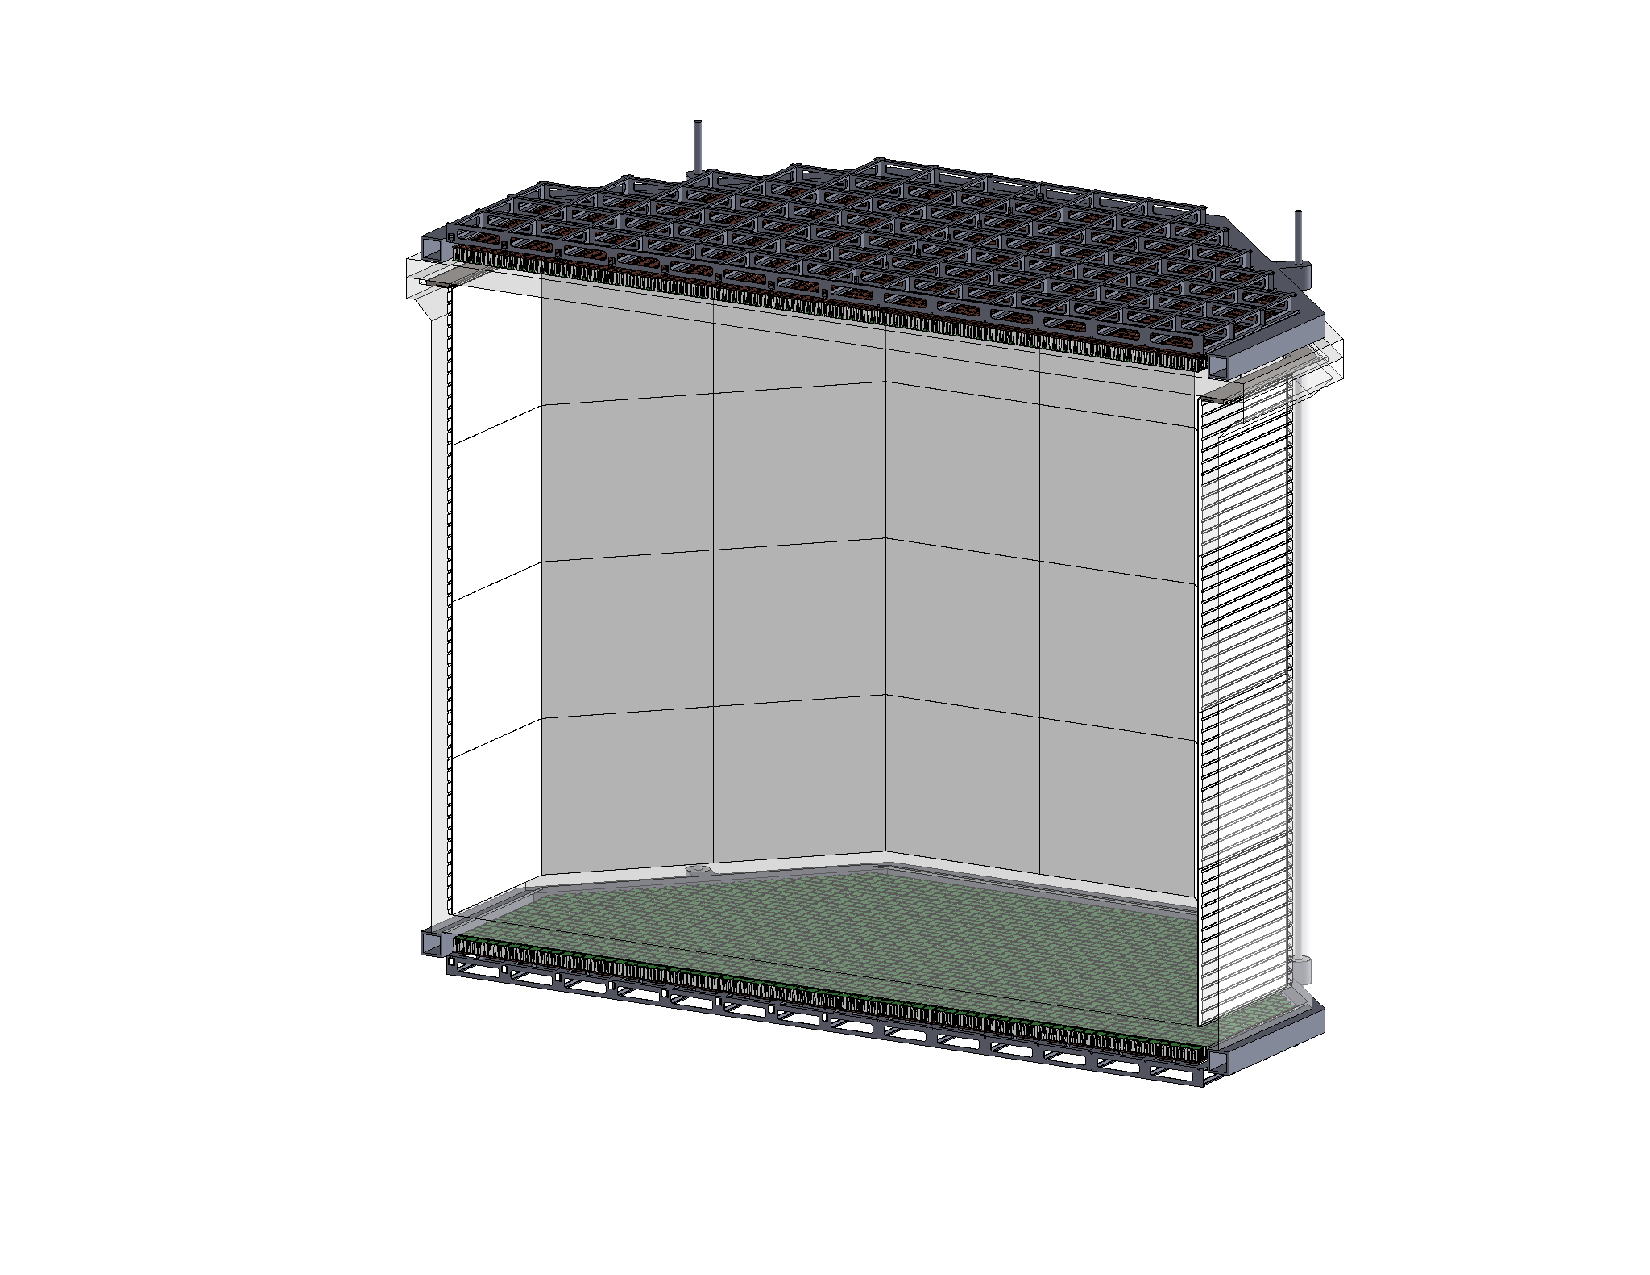
\includegraphics[width=\columnwidth]{./Figures/TPC-acrylic-vessel-design.pdf}
\caption{3D model of the \TPC\ with acrylic vessel.}
\label{fig:TPC_acrylic}
\end{figure}